%%% The main file. It contains definitions of basic parameters and includes all other parts.

%% Settings for single-side (simplex) printing
% Margins: left 40mm, right 25mm, top and bottom 25mm
% (but beware, LaTeX adds 1in implicitly)
\documentclass[12pt,a4paper]{report}
\setlength\textwidth{145mm}
\setlength\textheight{247mm}
\setlength\oddsidemargin{15mm}
\setlength\evensidemargin{15mm}
\setlength\topmargin{0mm}
\setlength\headsep{0mm}
\setlength\headheight{0mm}
% \openright makes the following text appear on a right-hand page
\let\openright=\clearpage

%% Settings for two-sided (duplex) printing
% \documentclass[12pt,a4paper,twoside,openright]{report}
% \setlength\textwidth{145mm}
% \setlength\textheight{247mm}
% \setlength\oddsidemargin{14.2mm}
% \setlength\evensidemargin{0mm}
% \setlength\topmargin{0mm}
% \setlength\headsep{0mm}
% \setlength\headheight{0mm}
% \let\openright=\cleardoublepage

%% Generate PDF/A-2u
\usepackage[a-2u]{pdfx}

%% Character encoding: usually latin2, cp1250 or utf8:
\usepackage[utf8]{inputenc}

%% Prefer Latin Modern fonts
\usepackage{lmodern}

%% Further useful packages (included in most LaTeX distributions)
\usepackage{amsmath}        % extensions for typesetting of math
\usepackage{amsfonts}       % math fonts
\usepackage{amsthm}         % theorems, definitions, etc.
\usepackage{bbding}         % various symbols (squares, asterisks, scissors, ...)
\usepackage{bm}             % boldface symbols (\bm)
\usepackage{graphicx}       % embedding of pictures
\usepackage{fancyvrb}       % improved verbatim environment
\usepackage{natbib}         % citation style AUTHOR (YEAR), or AUTHOR [NUMBER]
\usepackage[nottoc]{tocbibind} % makes sure that bibliography and the lists
			    % of figures/tables are included in the table
			    % of contents
\usepackage{dcolumn}        % improved alignment of table columns
\usepackage{booktabs}       % improved horizontal lines in tables
\usepackage{paralist}       % improved enumerate and itemize
\usepackage{xcolor}         % typesetting in color

%%% Basic information on the thesis

% Thesis title in English (exactly as in the formal assignment)
\def\ThesisTitle{Document embedding using Transformers}

% Author of the thesis
\def\ThesisAuthor{David Burian}

% Year when the thesis is submitted
\def\YearSubmitted{2023}

% Name of the department or institute, where the work was officially assigned
% (according to the Organizational Structure of MFF UK in English,
% or a full name of a department outside MFF)
\def\Department{Institute of Formal and Applied Linguistics}

% Is it a department (katedra), or an institute (ústav)?
\def\DeptType{Institute}

% Thesis supervisor: name, surname and titles
\def\Supervisor{Jindřich, Libovický Mgr. Ph.D.}

% Supervisor's department (again according to Organizational structure of MFF)
\def\SupervisorsDepartment{Institute of Formal and Applied Linguistics}

% Study programme and specialization
\def\StudyProgramme{Computer Science}
\def\StudyBranch{Artificial Inteligence}

% An optional dedication: you can thank whomever you wish (your supervisor,
% consultant, a person who lent the software, etc.)
\def\Dedication{%
Dedication.
}

% Abstract (recommended length around 80-200 words; this is not a copy of your thesis assignment!)
\def\Abstract{%
Abstract.
}

% 3 to 5 keywords (recommended), each enclosed in curly braces
\def\Keywords{%
  {text embedding} {document embedding} {transformers} {document
  classification} {document similarity}
}

%% The hyperref package for clickable links in PDF and also for storing
%% metadata to PDF (including the table of contents).
%% Most settings are pre-set by the pdfx package.
\hypersetup{unicode}
\hypersetup{breaklinks=true}

% Definitions of macros (see description inside)
%%% This file contains definitions of various useful macros and environments %%%
%%% Please add more macros here instead of cluttering other files with them. %%%

%%% Minor tweaks of style

% These macros employ a little dirty trick to convince LaTeX to typeset
% chapter headings sanely, without lots of empty space above them.
% Feel free to ignore.
\makeatletter
\def\@makechapterhead#1{
  {\parindent \z@ \raggedright \normalfont
   \Huge\bfseries \thechapter. #1
   \par\nobreak
   \vskip 20\p@
}}
\def\@makeschapterhead#1{
  {\parindent \z@ \raggedright \normalfont
   \Huge\bfseries #1
   \par\nobreak
   \vskip 20\p@
}}
\makeatother

% This macro defines a chapter, which is not numbered, but is included
% in the table of contents.
\def\chapwithtoc#1{
\chapter*{#1}
\addcontentsline{toc}{chapter}{#1}
}

% Draw black "slugs" whenever a line overflows, so that we can spot it easily.
\overfullrule=1mm

%%% Macros for definitions, theorems, claims, examples, ... (requires amsthm package)

\theoremstyle{plain}
\newtheorem{thm}{Theorem}
\newtheorem{lemma}[thm]{Lemma}
\newtheorem{claim}[thm]{Claim}

\theoremstyle{plain}
\newtheorem{defn}{Definition}

\newtheorem{repre_prop}{Property}

\theoremstyle{remark}
\newtheorem*{cor}{Corollary}
\newtheorem*{rem}{Remark}
\newtheorem*{example}{Example}

%%% An environment for proofs

\newenvironment{myproof}{
  \par\medskip\noindent
  \textit{Proof}.
}{
\newline
\rightline{$\qedsymbol$}
}

%%% An environment for typesetting of program code and input/output
%%% of programs. (Requires the fancyvrb package -- fancy verbatim.)

\DefineVerbatimEnvironment{code}{Verbatim}{fontsize=\small, frame=single}

%%% The field of all real and natural numbers
\newcommand{\R}{\mathbb{R}}
\newcommand{\N}{\mathbb{N}}

%%% Useful operators for statistics and probability
\DeclareMathOperator{\pr}{\textsf{P}}
\DeclareMathOperator{\E}{\textsf{E}\,}
\DeclareMathOperator{\var}{\textrm{var}}
\DeclareMathOperator{\sd}{\textrm{sd}}

%%% Transposition of a vector/matrix
\newcommand{\T}[1]{#1^\top}

%%% Various math goodies
\newcommand{\goto}{\rightarrow}
\newcommand{\gotop}{\stackrel{P}{\longrightarrow}}
\newcommand{\maon}[1]{o(n^{#1})}
\newcommand{\abs}[1]{\left|{#1}\right|}
\newcommand{\dint}{\int_0^\tau\!\!\int_0^\tau}
\newcommand{\isqr}[1]{\frac{1}{\sqrt{#1}}}
\DeclareMathOperator*{\argmin}{\arg\!\min\medspace}
\DeclareMathOperator*{\argmax}{\arg\!\max\medspace}

%%% Various table goodies
\newcommand{\pulrad}[1]{\raisebox{1.5ex}[0pt]{#1}}
\newcommand{\mc}[1]{\multicolumn{1}{c}{#1}}


% Title page and various mandatory informational pages
\begin{document}
%%% Title page of the thesis and other mandatory pages

%%% Title page of the thesis

\pagestyle{empty}
\hypersetup{pageanchor=false}
\begin{center}

\centerline{\mbox{
\includegraphics[width=166mm]{./img/logo-en.pdf}}}

\vspace{-8mm}
\vfill

{\bf\Large MASTER THESIS}

\vfill

{\LARGE\ThesisAuthor}

\vspace{15mm}

{\LARGE\bfseries\ThesisTitle}

\vfill

\Department

\vfill

{
\centerline{\vbox{\halign{\hbox to 0.45\hsize{\hfil #}&\hskip 0.5em\parbox[t]{0.45\hsize}{\raggedright #}\cr
Supervisor of the master thesis:&\Supervisor \cr
\noalign{\vspace{2mm}}
Study programme:&\StudyProgramme \cr
\noalign{\vspace{2mm}}
Study branch:&\StudyBranch \cr
}}}}

\vfill

% Zde doplňte rok
Prague \YearSubmitted

\end{center}

\newpage

%%% Here should be a bound sheet included -- a signed copy of the "master
%%% thesis assignment". This assignment is NOT a part of the electronic
%%% version of the thesis. DO NOT SCAN.

%%% A page with a solemn declaration to the master thesis

\openright
\hypersetup{pageanchor=true}
\pagestyle{plain}
\pagenumbering{roman}
\vglue 0pt plus 1fill

\noindent
I declare that I carried out this master thesis independently, and only with the cited
sources, literature and other professional sources. It has not been used to obtain another
or the same degree.

\medskip\noindent
I understand that my work relates to the rights and obligations under the Act No.~121/2000 Sb.,
the Copyright Act, as amended, in particular the fact that the Charles
University has the right to conclude a license agreement on the use of this
work as a school work pursuant to Section 60 subsection 1 of the Copyright~Act.

\vspace{10mm}

\hbox{\hbox to 0.5\hsize{%
In \hbox to 6em{\dotfill} date \hbox to 6em{\dotfill}
\hss}\hbox to 0.5\hsize{\dotfill\quad}}
\smallskip
\hbox{\hbox to 0.5\hsize{}\hbox to 0.5\hsize{\hfil Author's signature\hfil}}

\vspace{20mm}
\newpage

%%% Dedication

\openright

\noindent
\Dedication

\newpage

%%% Mandatory information page of the thesis

\openright

\vbox to 0.5\vsize{
\setlength\parindent{0mm}
\setlength\parskip{5mm}

Title:
\ThesisTitle

Author:
\ThesisAuthor

\DeptType:
\Department

Supervisor:
\Supervisor, \SupervisorsDepartment

Abstract:
\Abstract

Keywords:
\Keywords

\vss}

\newpage

\openright
\pagestyle{plain}
\pagenumbering{arabic}
\setcounter{page}{1}


%%% A page with an automatically generated table of contents of the master thesis

\tableofcontents

%%% Each chapter is kept in a separate file
\chapter*{Introduction}
\addcontentsline{toc}{chapter}{Introduction}



\chapter{Related Work}

- approaches so far: the `history'

\chapter{Benchmarks}

In this chapter we will describe a set of benchmarks, which will test our model
and enable us to compare it to other models. First we will describe the tasks
--- datasets and corresponding evaluation metrics, then we will talk about the
models. Results of the benchmarks are discussed in
Chapter~\ref{chapter:evaluation}.

\section{Tasks}

Each task aims to test a different aspect of a model. Our aim was to design a
set of tasks, which can capture a model's capability to embed whole documents.
The major obstacle we faced was the lack of labeled datasets with longer pieces
of text (more than 512 tokens).

TODO: how did we solve the issue

TODO: complete list of task types

\subsubsection{Classification}

Classification tasks test model's capability to separate inputs based on a
complex feature. In our settings, classification tasks can tell us what
information the document embedding contains.


\subsection{IMDB Sentiment Analysis}

IMDB sentiment analysis task is a simple binary classification task. The dataset
contains movie reviews from the Internet Movie
Database\footnote{\url{www.imdb.com}} labaled as either positive or negative.
The dataset is commonly referred to as IMDB classification or sentiment
dataset~\cite{maas11}.

The dataset is split evenly to test and train set, each having 25000 reviews.
The dataset also contains 50000 unlabeled reviews. The label distribution in
both sets is uniform, each of of the two labels is represented by 12500 reviews.

As can be seen from the figure Figure~\ref{fig:imdb_word_token_dist} the reviews
are quite short with only 13.56\% being longer than 512 RoBERTa tokens.

\begin{figure}[ht]
  \centering
  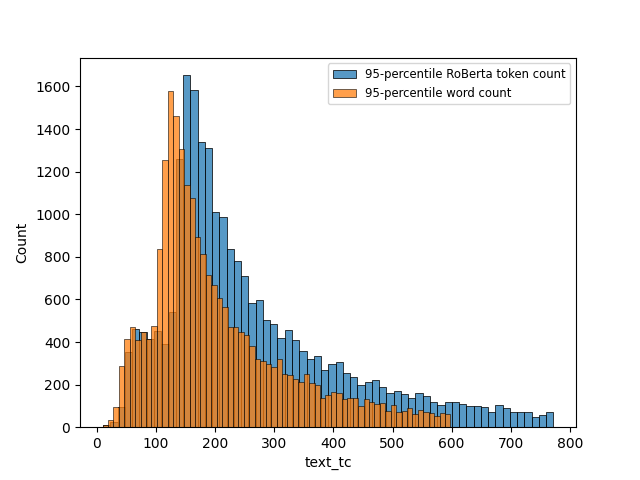
\includegraphics[width=0.9\textwidth]{img/imdb_word_token_distributions.png}
  \caption{Word count and token count distribution of 95-percentiles of
  reviews. The tokens are generated using RoBERTa's pretrained tokenizer from
  HuggingFace}\label{fig:imdb_word_token_dist}
\end{figure}

We included this task to see how our model compares in realtively undemanding
settings, while also evaluating its performence on shorter documents.

\section{Models}

In this section we describe a set of benchmark models our model will be compared
to. All of the benchmark models are able to map a continuous piece of text to a
dense vector representation. This was a requirement as the aim of the evaluation
is to compare different text embeddings. Otherwise we aimed to select a variety
of models with different architectures, learning algorithms and learning tasks.

\subsection{Paragraph Vector}

Paragraph Vector (also known as Doc2Vec) introduced in \cite{le2014distributed},
combines slightly altered DBOW and DM architectures previously used by Word2Vec
in \cite{mikolov2013efficient}. As seen in Figure~\ref{fig:pv-dm_pv-dbow} the
model's versions of DBOW and DM architectures, called PV-DBOW and PV-DM,
incorporate paragraph's identifier. This allows the architectures to store the
information about the input paragrahs, which is then used as the paragraph's
embedding. The final paragrpah embedding is linear combination of the
representations of both architectures. Note that, a paragrpah can be any piece
of continuous text.

TODO: my own graphic here

\begin{figure}[h]
    \centering
    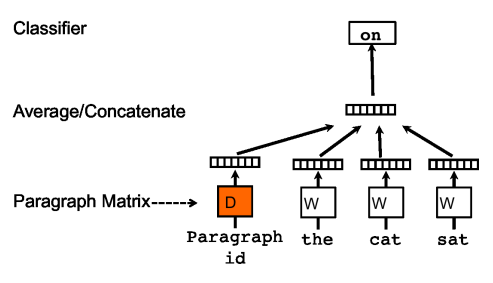
\includegraphics[width=0.4\textwidth]{./img/pv-dm.png}
    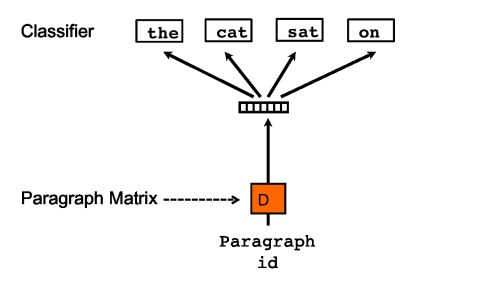
\includegraphics[width=0.4\textwidth]{./img/pv-dbow.png}
    \caption{PV-DM and PV-DBOW architectures.\label{fig:pv-dm_pv-dbow}}
\end{figure}

Paragraph Vector is trained using language modelling --- both architectures should
predict a word which is probable in the given context. In PV-DM the context is
paragraph id and the neighbouring words, in PV-DBOW the context is only the
pragraph id.

Paragraph Vector's advantage is its small size and therefore quick learning.
Moreover it is able to process paragraphs of all lengths. The disadvantage is
that the embedding must be learned even during inference.

\subsection{SBERT}

Sentence-BERT (or SBERT for short) introduced in \cite{reimers2019sentence}, is
a composition of a BERT-like model with pooling layer above its final hidden
states. This architecture is common for sequence classification using a
transformer model. SBERT differs from these simpler approaches, by finetuning on
NLI datasets using siamiese networks. The training setup is depicted in
Figure~\ref{fig:sbert_siemese}. After such training the STS scores of SBERT
embeddings significantly increases.

\begin{figure}
    \centering
    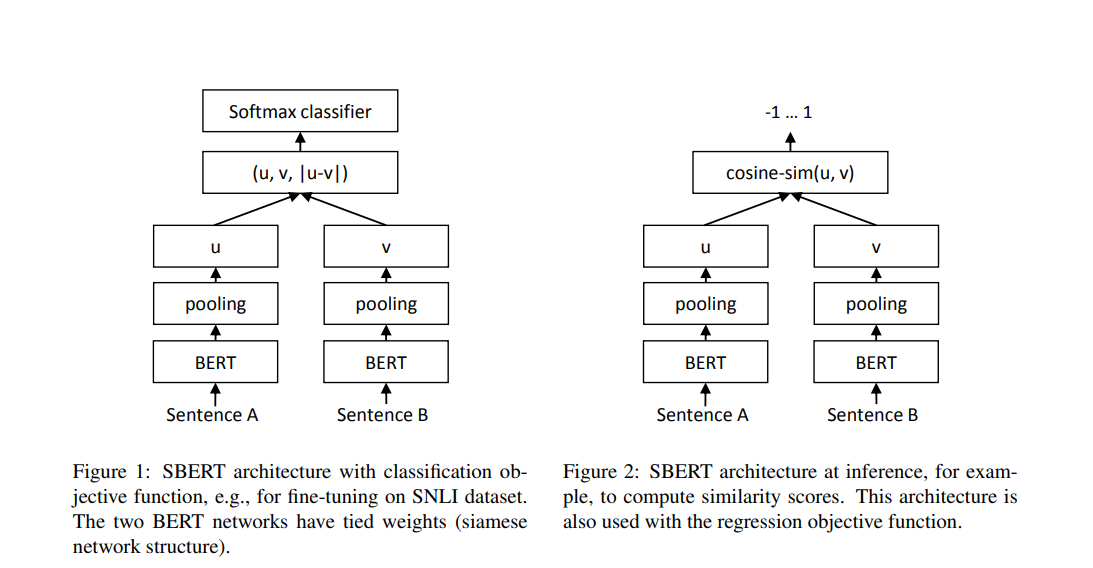
\includegraphics[width=0.9\textwidth]{./img/sbert_pairs_architectures.png}
    \caption{SBERT architecture with siamiese
    networks.\label{fig:sbert_siemese}}
\end{figure}

The disadvantage of SBERT is its inability to process longer pieces of texts.
The workaround is to either truncate the input or to average multiple embeddings
produced by a sliding window over the input. Both approaches limit the model's
ability to see the document as a whole, which could impair the quality of the
produced embeddings.

\subsection{Longformer}

Longformer introduced in \cite{beltagy2020longformer}, is a transformer with
sparse attention matrix. Whereas in traditional transformer we see dense
attention matrix --- every token ``attends'' to every other token, in
Longformer's attention every token ``attends'' only to selected few global
tokens and neighbouring tokens. Example of such sparse attention matrix is
depicted in Figure~\ref{fig:longformer_sparse_att}. This allows Longformer to
process inputs in linear time of the input length. Thus Longformer is able to
process inputs up to 4096 tokens long.

TODO: maybe comparison to normal dense attention

\begin{figure}[h]
    \centering
    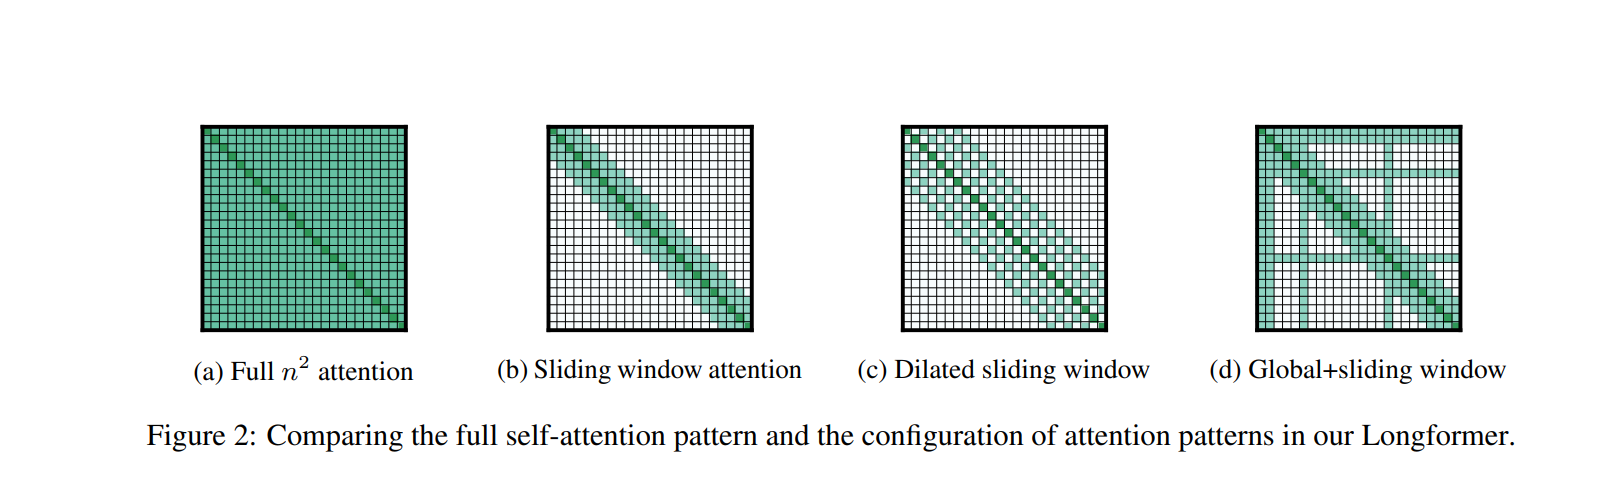
\includegraphics[width=0.9\textwidth]{./img/longformer_attention.png}
    \caption{Longformer attention matrix.\label{fig:longformer_sparse_att}}
\end{figure}

While sparse attention matrix allows Longformer to process longer texts, it also
limits its computational power. \cite{zaheer2020big} show that with sparse
attention we need more layers to match the power of a dense attention matrix.

To produce input embeddings we average the embeddings of last hidden states.

TODO: training

\subsection{BigBird}

TODO: how is it different from longformer





\chapter{Distilling structural and contextual qualities of document
embeddings}\label{chapter:training_method}

In this chapter, we introduce our method of training document embeddings. We
base our approach on teacher-student training, distilling the knowledge of two
embedding models (referred to as \emph{teachers}) into one  \emph{student}
model. Section~\ref{section:training_method} explains our training method in
detail and outlines the used loss function. In the rest of this chapter, we
describe the two teacher models in Section~\ref{section:teacher_models} and the
student in Section~\ref{section:student_model}.

\section{Training methodology}\label{section:training_method}

Our training methodology aims to train an embedding model such that its
embeddings more faithfully represent the input. As we describe in
Chapter~\ref{chapter:document_representation}, we distinguish two qualities of
faithful representations: structural and contextual. The goal is to instill
both qualities into a single embedding model. To do so, we use teacher-student
training with two teacher embedding models, one with high structural capacity
and the other with high contextual capacity.

In the following subsections, we describe teacher-student training in detail
and give a high-level overview of the proposed loss function.

\subsection{Teacher-student training}

In the teacher-student training, we train a student model based on a frozen
teacher model. The goal is to make the student model imitate the teacher model,
thereby digesting the teacher's understanding of the input. Although the
student model is generally not expected to outperform the teacher model,
teacher-student training is still valuable in several situations. For instance,
\cite{sanh2019distilbert} use teacher-student training to make a model smaller
while sacrificing only a fraction of its performance. In another scenario,
\cite{reimers2020making} use teacher-student training to enforce similarity
between models' outputs, thereby giving the student model a powerful training
signal.

We assume two embedding models in our setting: a structural teacher
$\Teacher_S$ and a contextual teacher $\Teacher_C$ with high structural and
contextual capacities, respectively. Teacher-student training allows us to
instill both capacities into a third student model {\Student} while avoiding
the architectural limitations of the teachers. We hypothesize that we can
efficiently direct the two training signals so that they do not push against
each other.


\subsection{Abstract loss formulation}\label{section:abstract_loss}


We instill a quality of a teacher's embedding by simply enforcing a similarity
between the teacher's and student's embedding. Since we have two teachers, we
use two similarities $\Loss_S$, and $\Loss_C$, which compare the student's
embedding $y_\Student$ with the structural teacher's embedding $y_{\Teacher_S}$
and the contextual teacher's embedding $y_{\Teacher_C}$, respectively. We show
a graphical overview of the training architecture in
Figure~\ref{fig:teacher_student_train_arch}.

To regulate the mixture of $\Loss_S$ and $\Loss_C$, we introduce weighting
parameter $\lambda$. In the most general form, we assume $\lambda$ to be
dependent on the input text $x$ since the performance of the teacher models
might vary across different inputs. In particular, we can expect $\lambda$ to
depend on the length of the input since, for shorter inputs, the context
is minimal and, therefore, expendable. Abstract formulation of the loss is
given in Equation~\ref{eq:abstract_loss}. We explore concrete options for
$\Loss_S$, $\Loss_C$ and $\lambda(x)$ in Chapter~\ref{chapter:experiments}.

\begin{equation}\label{eq:abstract_loss}
  \Loss(
    x,
    y_\Student,
    y_{\Teacher_S},
    y_{\Teacher_C},
    \lambda
  ) =
    \lambda(x) \Loss_S(y_\Student, y_{\Teacher_S}) +
            (1 - \lambda(x)) \Loss_C(y_\Student, y_{\Teacher_S})
\end{equation}

The two losses could push against each other and slow down or halt the
training. To avoid that, we choose one of the losses to be more strict while
the other to be more forgiving. In that way, the more forgiving loss should
adapt to the strict one instead of pushing against it. As mentioned in
Section~\ref{section:combine_structural_and_contextual}, we view structural
quality as the more important. Therefore, we choose the structural loss
$\Loss_S$ as the stricter and exact loss, forcing the student to mimic the
structural teacher as much as possible. On the other hand, the contextual loss
$\Loss_C$ should give the student model more freedom in the form of the
produced embedding but still force it to incorporate the information from the
contextual embedding.

\begin{figure}
  \centering
  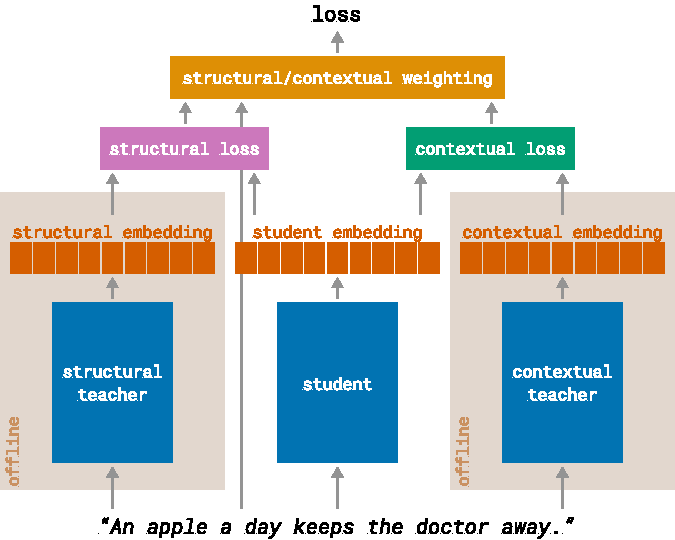
\includegraphics[width=0.8\textwidth]{./img/training_architecture.pdf}

  \caption{The architecture of our teacher-student training. We distill the
  qualities of the teachers' embeddings through corresponding losses into a
  student model. Since we do not update the weights of either teacher,
  the generation of their embeddings can be done offline before training.}

  \label{fig:teacher_student_train_arch}

\end{figure}

\section{Teacher models}\label{section:teacher_models}

This section introduces the teacher models used during our experiments in
Chapter~\ref{chapter:experiments}. We chose Sentence-BERT
\citep{reimers2019sentence} as the structural teacher model and Paragraph
Vector \citep{le2014distributed} (or \emph{PV}) as the context teacher model.
As explained in Chapter~\ref{chapter:document_representation}, each of the two
mentioned models specializes in a different quality of produced embeddings.
SBERT can compare word relationships on many levels and thus understand even
complex text structures. However, it cannot process long texts. On the other
hand, Paragraph Vectors can produce embeddings even for long documents, but they
process text very shallowly, which prohibits understanding any complex
structures. We hope to synthesize both qualities by combining the two
teacher models in a single model.

\subsection{SBERT}

Sentence-BERT is a composition of a BERT-like \citep{devlin2019bert} encoder
with a mean pooling layer above its last layer's hidden states. The model is
finetuned with Natural Language Inference (\emph{NLI}) datasets to produce
semantically meaningful embeddings. We illustrate SBERT's training
architecture in Figure~\ref{fig:sbert}. We have chosen SBERT as a structural
teacher for its high structural capacity and strong performance in
sentence-level text-understanding tasks \citep{reimers2019sentence}.

\begin{figure}
  \centering
  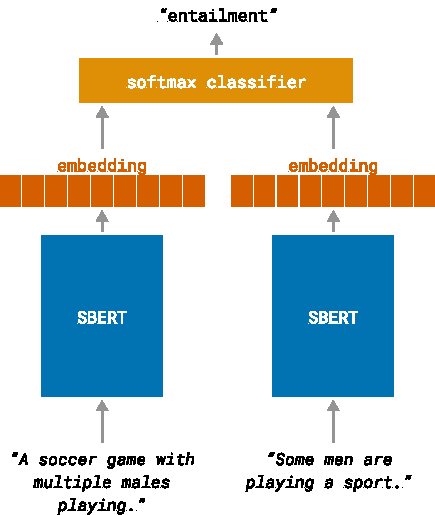
\includegraphics[width=0.5\textwidth]{./img/sbert_architecture.pdf}

  \caption{Siamese network architecture used to train SBERT. The pair of
  sentences from an NLI dataset is classified into three classes
  ``entailment'', ``neutral'' and ``contradiction''.}

  \label{fig:sbert}

\end{figure}

\subsection{Paragraph Vector}\label{section:paragraph_vector}

Paragraph Vector \citep{le2014distributed}, sometimes referred to as Doc2Vec, is a simple
text-embedding model that views the input as a Bag of Words (or BoW). Paragraph
Vector comprises two sub-models: Distributed Memory (DM) and Distributed Bag of
Words (DBOW). While each model is trained separately, the authors recommend combining both architectures into a single model, where the combined models' embeddings are simply concatenated. The models are trained to
predict a word within a window in the given document. As shown in
Figure~\ref{fig:dbow}, DBOW bases its prediction only on the whole paragraph's embedding. On the other hand, DM, whose architecture is depicted in
Figure~\ref{fig:dm}, additionally uses the embeddings of the surrounding words
within a given window.

We chose Paragraph Vector as a contextual teacher due to its unique
architecture, which forces the model to develop a single vector that summarizes
the common theme of the document. Moreover, Paragraph Vector does not have a
limited maximum input length, so as a contextual teacher, it will always
provide some signal to the student regarding the document's context. Also, even
though Paragraph Vector cannot match the performance of substantially more
complex models such as Transformers, \cite{dai2015document} show that for
larger datasets, Paragraph Vector, outperforms classical embedding models such
as Latent Dirichlet Allocation \citep{blei2003latent} or TF-IDF weighted BoW
model \citep{harris1954distributional}. Finally, Paragraph Vector's simple
architecture allows it to train on significantly larger text corpora than other
bigger models, such as SBERT. Therefore, for a given computational budget,
Paragraph Vector would see more documents during training than SBERT, which may
give it a slight advantage.

\begin{figure}
  \centering
  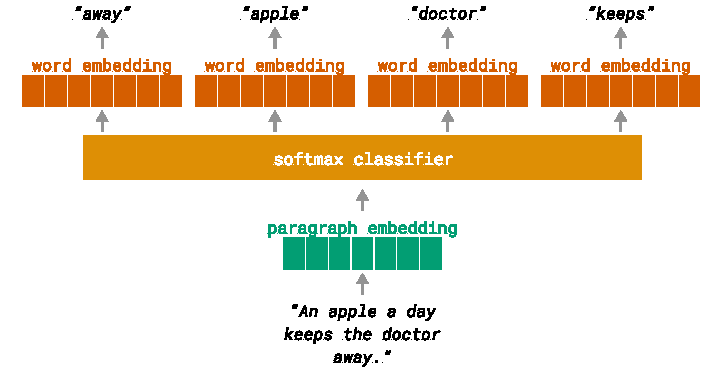
\includegraphics[width=0.8\textwidth]{./img/dbow_architecture.pdf}

  \caption{Architecture of Distributed Bag of Words. The model predicts words
  from a document, only using the document's embedding.}

  \label{fig:dbow}
\end{figure}

\begin{figure}
  \centering
  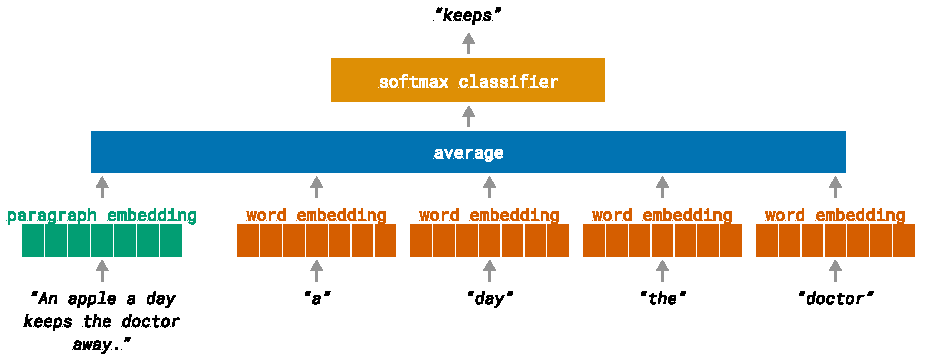
\includegraphics[width=1\textwidth]{./img/dm_architecture.pdf}

  \caption{Distributed Memory model architecture. The model predicts the input
  words' neighboring word for the input paragraph.}

  \label{fig:dm}

\end{figure}

\section{Student model}\label{section:student_model}

In our teacher-student training, the student model is our primary embedding
model, which we train based on the outputs of the teacher models. By using
teacher-student training, we can avoid some of the architectural drawbacks of
both teacher models while still benefiting from the qualities of the teachers'
embeddings. We choose the student's architecture at a midpoint between
the two teachers' architectures. In other words, not to be as complex as the
architecture of SBERT, so it can process longer inputs while still having a
manageable memory footprint, but not as simple as the architecture of PV, so
that the student can model complex world relationships. We chose a Transformer
with a sparse attention mechanism. Transformer is a well-tested architecture
that is used throughout NLP. Additionally, with sparse attention, Transformers
consume a relatively small amount of memory even for longer inputs, as we
explain in Section~\ref{section:efficient_self_attn}. Another consideration is
that we need a pre-trained model, as our method is not suited to train a model
from scratch but to finetune a model's document embeddings.

Contrary to the selection of architecture, selecting a concrete model is not
crucial to our method. Our choice of the concrete model is governed more by
practical considerations rather than the conditions of our method. Since we
have limited computational resources, we prefer a smaller model that we can fit
on a consumer-grade GPU card. We also value the model's performance, ease of
use, and simplicity. We choose Longformer \citep{beltagy2020longformer} as it
is reasonably small, memory efficient, performs above average compared to other
similar models \citep{tay2020long}, and its self-attention mechanism is
straightforward. Other alternatives are BigBird \citep{zaheer2020big}, or if we
would not mind a more complex model, we could use Reformer
\citep{kitaev2020reformer}, Linformer \citep{wang2020linformer} or Performer
\citep{choromanski2020rethinking}.

\subsection{Longformer}

Longformer \citep{beltagy2020longformer} is a Transformer encoder with sparse
attention. Because we refer to Longformer's configuration and training in the
following chapters, we briefly explain Longformer's self-attention mechanism
and the training data of the pre-trained checkpoint.


\subsubsection{Self-attention mechanism}

Longformer has a sparse self-attention mechanism that composes three different
patterns: local, global, and dilated local attention. Local attention is simply
full attention but only within the neighborhood of $\frac{1}{2}\omega$ tokens
on either side of the key token. $\omega$ can be set differently per
self-attention layer. In global attention, few selected tokens attend to all
other tokens. The tokens on which Longformer computes global attention can be
selected per each input. Global attention's parameters are not pre-trained.
Instead, at the beginning of the training, they are initialized by the
parameters from local attention and finetuned for a given task. With dilated
local attention, every key token attends to every $k$ neighboring query token.
So, it is analogous to a one-dimensional Convolution layer
\citep{van2016wavenet} with stride, or dilatation of $k$. However, to use
dilated local attention, one has to use a custom CUDA kernel or a slow
implementation in Python using loops. The authors also provide a reasonably
fast, memory-efficient block implementation for global and local
attention.

\subsubsection{Training}

Longformer is warm-started from a RoBERTa \citep{liu2019roberta} checkpoint
with its learned positional embeddings duplicated eight times to support inputs
up to 4096 tokens long. The authors show that duplicating RoBERTa's positional
embeddings is faster than training position embeddings for all 4096 positions
from scratch. Then, the authors train Longformer using MLM on long documents
for 65k gradient steps to improve its capabilities for longer inputs. The
training corpus overlaps with RoBERTa's pretraining corpus but is more focused
on longer pieces of text. It includes the following datasets:

\begin{itemize}

  \item Book corpus \citep{zhu2015aligning}

  \item English Wikipedia

  \item One-third of articles from Realnews dataset \citep{zellers2019defending}
      with more than 1200 tokens

  \item One-third of the Stories corpus \citep{trinh2018simple}

\end{itemize}

Unfortunately, as of this writing, the Book corpus is unavailable due to
licensing issues. Moreover, we have not been able to find a comparable
alternative. The Stories corpus is also unavailable. However, there is an
alternative\footnote{\url{https://huggingface.co/datasets/spacemanidol/cc-stories}}
that tries to mimic the dataset from the original paper.

\chapter{Evaluation}\label{chapter:evaluation}

In this chapter, we evaluate the most promising configurations of our training
method. We train three student models on 1M documents with the best-performing
hyperparameters from Chapter~\ref{chapter:experiments} to show the effects of
long training with our teacher-student method. We evaluate the student models
on six classification and two retrieval tasks. For classification tasks, we
consider three different limits on the amount of available supervised data. We
show the models' performances vary for different limits and thus highlight
the strengths and limitations of our training method.

\section{Student models}

We only evaluate the three best-performing variants of our training method from
Chapter~\ref{chapter:experiments}. We use the hyperparameters listed in Table~\ref{table:experiments_final_config}, however, as we train the student models and the contextual teachers on significantly
more data, we label the models differently. {\CosineStudent}
is trained with a balanced mix of contextual loss and cosine structural loss,
which is masked out for inputs longer than the structural teacher's maximum
context length. {\MSEStudent} is trained with an equal mixture of contextual
loss and a max-margin MSE structural loss. Finally, {\OnlyMSEStudent} is
trained only on the max-margin MSE structural loss. These models'
hyperparameters correspond to the configurations of
\Model{masked-cosine;$\lambda$=0.5}, \Model{mm-MSE;$\lambda$=0.5}, and
\Model{only-structural;mm-MSE} from Table~\ref{table:experiments_final_config},
respectively.

\subsection{Training data}

We compile our training corpus the same as \Dataset{val-500k}. We train the
student models only using Longformer's training data. Without any new training
data, the performance of our student model depends only on our training
method. Hence, the performances of the student models are proportional to our
training method's performance, which gives us an easy way to gauge the benefits of our training method.

Following Longformer's approach, we equally sample articles from the English
Wikipedia\footnote{\url{https://huggingface.co/datasets/wikipedia/viewer/20220301.en}}
and documents from the RealNews dataset \citep{zellers2019defending} that have
above 1200 Longformer's tokens. We label the resulting dataset as
\Dataset{train-1M} and display its statistics in
Table~\ref{table:train_data_stats}. \Dataset{train-1M} contains relatively long
documents. The average document has around 1300 tokens, and only 34\% of its
documents can fit into the maximum context length of a vanilla Transformer.
However, as we show in Figure~\ref{fig:train_data_dist}, most documents have
between 0 and 500 tokens or 1200 and 1700 tokens.

\begin{table}
    \centering
    \footnotesize
\begin{tabular}{lrr}
\toprule
Split & Train & Validation \\
\midrule
Documents & 1 000 000 & 30 000 \\
Tokens & 1.37e+09 & 4.15e+07 \\
Tokens per document & 1375$\pm$1738 & 1382$\pm$1697 \\
SBERT tokens over 384 & 71\% & 71\% \\
SBERT tokens over 512 & 66\% & 67\% \\
\bottomrule
\end{tabular}


    \caption{Statistics of \Dataset{train-1M}. For each split, we also show
    the percentage of documents with the number of SBERT tokens above the given
    threshold.}

    \label{table:train_data_stats}

\end{table}

\begin{figure}
    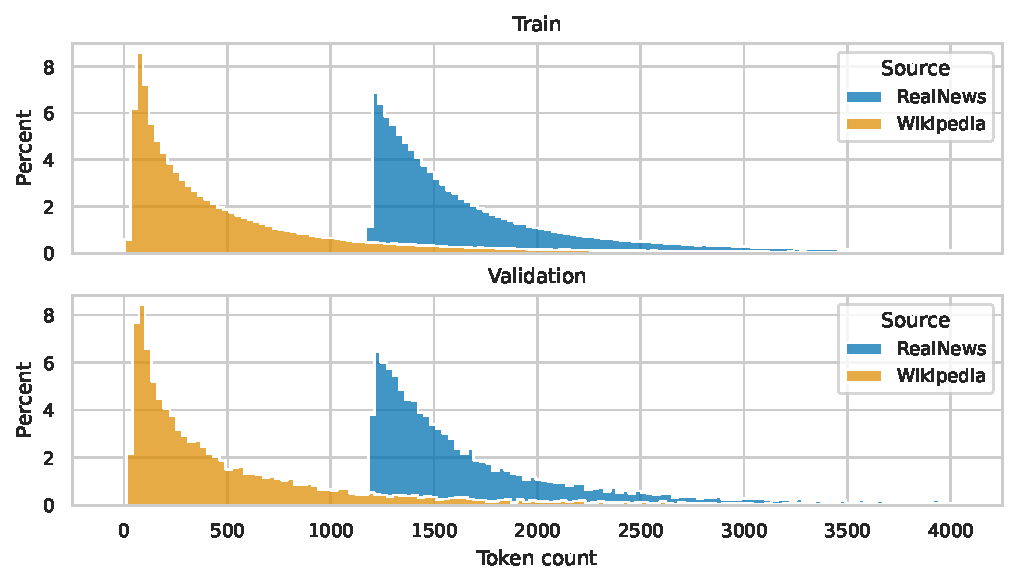
\includegraphics[width=\textwidth]{./img/train_data_dist.pdf}

    \caption{Distribution of the number of Longformer tokens per document in
    \Dataset{train-1M}.}

    \label{fig:train_data_dist}
\end{figure}


\subsection{Training of contextual teachers}

Two of our student models use a contextual teacher. To showcase the full
potential of our training method, we train the contextual teachers anew and
with much more data than in the previous chapter. {\CosineStudent} uses a
2048-dimensional Paragraph Vector \citep{le2014distributed} composed of
Distributed Memory and Distributed Bag of Words models. {\MSEStudent} uses only
a 100-dimensional Distributed Memory model. These contextual teachers correspond to \Model{PV;2048d} and \Model{DM;100d} from Section~\ref{section:pv_training} respectively.

We compile the contextual teacher's training dataset in the same manner as
\Dataset{train-1M}. Since the contextual teachers' training
data also becomes the student's training data, we restrict it to Longformer's training data for the
reasons we mention in the previous section. However, as PV is a significantly
smaller model than our student model, we can afford to train it with
substantially more data. We use all available data from RealNews articles and
an equal amount of Wikipedia documents. The resulting dataset has 8.3 million
documents. We label the trained 100-dimensional and 2048-dimensional teachers
\Model{DM} and \Model{PV}. To keep the models' memory footprint manageable, we
restrict \Model{DM}'s vocabulary to $6\times 10^7$ words and \Model{PV}'s
vocabulary to $1.2\times 10^7$ words. With these limitations, the models take
up approximately 96GB and 124GB of memory during prediction.

\subsection{Training of student models}

Finally, we train the student models with the newly trained contextual teachers.
We train on \Dataset{train-1M} for one epoch with hyperparameters listed in
Table~\ref{table:final_student_train_params}. Thanks to the student's efficient
self-attention, the models take up only 12GB of VRAM during training. We train
the models on an NVIDIA A100 GPU card for approximately 30 hours.

\begin{table}
  \centering
  \footnotesize

  \begin{tabular}{l c}
    \toprule
    Parameter & Value \\
    \midrule
    Batch size & 6 \\
    Weight decay & 0.1 \\
    Learning rate & 3e-5 \\
    Learning rate decay & Cosine \\
    Maximum gradient norm & 1.0 \\
    Optimizer & AdamW \\
    Gradient accumulation steps & 10 \\
    Warmup update steps & 500\\
    Gradient checkpointing & Yes \\
    Mixed-precision training & Yes \\
    \bottomrule
  \end{tabular}

  \caption{Hyperparameters used for training all three student models:
  {\CosineStudent}, {\MSEStudent}, and {\OnlyMSEStudent}.}

  \label{table:final_student_train_params}

\end{table}

\section{Evaluation tasks}

We thoroughly evaluate the student models using eight diverse tasks. We
select six classification tasks that cover citation prediction, plagiarism
detection, sentiment, and topic classification. We also include two retrieval
tasks from distinct domains.

We present an overview of the selected classification tasks in
Table~\ref{table:eval_cls_tasks_overview}. Besides ordinary classification
tasks, we also include classifications of document pairs. In these tasks,
the classifier bases its prediction on the comparison of two documents, or in
our case,  their two embeddings. As can be seen from
Table~\ref{table:evaluation_tasks_stats}, the amount of the tasks' finetuning
and evaluation data ranges. This becomes particularly important in
Section~\ref{section:eval_cls_tasks}, where we evaluate the student models
while limiting the tasks' training data to different amounts.

\begin{table}
  \footnotesize
  \centering

  \begin{tabular}{llrrr}
      \toprule
      \multicolumn{3}{c}{} & \multicolumn{2}{c}{Class percentage $\sigma$} \\
      \cline{4-5}
      Dataset & Inputs & Classes & Train & Test \\
      \midrule
      \Task{arxiv} & documents & 11 & 1.25 & 1.30 \\
      \Task{imdb} & documents & 2 & 0.00 & 0.00 \\
      \Task{aan} & pairs of documents & 2 & 1.50 & 0.77 \\
      \Task{oc} & pairs of documents & 2 & 0.07 & 0.34 \\
      \Task{pan} & pairs of documents & 2 & 0.00 & 0.00 \\
      \Task{s2orc} & pairs of documents & 2 & 0.09 & 0.33 \\
      \bottomrule
  \end{tabular}

  \caption{Overview of the classification tasks. For each task, we include the
  type of input classified. The class distributions for all tasks are on
  average balanced, thus we show only the standard deviation of class
  percentages.}

  \label{table:eval_cls_tasks_overview}

\end{table}

\begin{table}
  \footnotesize
  \centering
    \begin{tabular}{llrrr}
        \toprule
        & & & \multicolumn{2}{c}{SBERT tokens} \\
        \cline{4-5}
        Dataset & Split & Documents & Over 384 & Over 512 \\
        \midrule
        \multirow[c]{2}{*}{\Task{arxiv}} & Train & 28 388 & 100\% & 100\% \\
        & Test & 2 500 & 100\% & 100\% \\
        \cline{1-5}
        \multirow[c]{2}{*}{\Task{imdb}} & Train & 25 000 & 25\% & 15\% \\
        & Test & 25 000 & 24\% & 14\% \\
        \cline{1-5}
        \multirow[c]{2}{*}{\Task{aan}} & Train & 106 592 & 0\% & 0\% \\
        & Test & 13 324 & 0\% & 0\% \\
        \cline{1-5}
        \multirow[c]{2}{*}{\Task{oc}} & Train & 240 000 & 12\% & 1\% \\
        & Test & 30 000 & 12\% & 1\% \\
        \cline{1-5}
        \multirow[c]{2}{*}{\Task{pan}} & Train & 17 968 & 70\% & 59\% \\
        & Test & 2 906 & 61\% & 47\% \\
        \cline{1-5}
        \multirow[c]{2}{*}{\Task{s2orc}} & Train & 152 000 & 33\% & 19\% \\
        & Test & 19 000 & 33\% & 18\% \\
        \cline{1-5}
        \bottomrule
    \end{tabular}

    \caption{Statistics of the classification tasks. We
    include the percentage of documents with SBERT tokens above a given
    threshold for each task and split.}

    \label{table:evaluation_tasks_stats}

\end{table}

We present an overview of the retrieval tasks in
Table~\ref{table:eval_sims_tasks}. These tasks do not have any finetuning data
and test only the proximity of embeddings of similar documents. Both tasks have
around 90 source articles, each with around eight similar target articles.
However, \Task{games} has substantially more documents.

\begin{table}
  \centering
  \footnotesize
  \begin{tabular}{lrrrrr}
    \toprule
    & & & & \multicolumn{2}{c}{SBERT tokens} \\
    \cline{5-6}
    Dataset & Documents & Sources & Targets per source & Over 384 & Over 512 \\
    \midrule
    \Task{wines} & 1 662 & 89 & 8.92$\pm$1.23 & 100\% & 90\% \\
    \Task{games} & 21 228 & 88 & 8.74$\pm$2.35 & 100\% & 92\% \\
    \bottomrule
  \end{tabular}

  \caption{Statistics of our similarity-based evaluation tasks. Each dataset
  has around 90 source documents, each similar to around nine target documents.
  We also include the percentage of documents with SBERT tokens above the given
  threshold.}

  \label{table:eval_sims_tasks}

\end{table}

We pay special attention to the lengths of documents contained in the datasets
and try to cover a span of lengths as large as possible. However, high-quality long document datasets are very rare due to their annotation's high complexity
and cost. Often, a dataset is said to be composed of documents, but it contains
only shorter pieces of text, such as abstracts. So, we include only one dataset
containing very long documents. As Figure~\ref{fig:eval_tasks_length_dist}
shows, the tasks arguably focus more on documents up to around 1024 tokens.
Nonetheless, as we show in
Tables~\ref{table:evaluation_tasks_stats}~and~\ref{table:eval_sims_tasks} the
tasks still contain a considerable number of documents longer than the maximum
context of our structural teacher.

\begin{figure}

    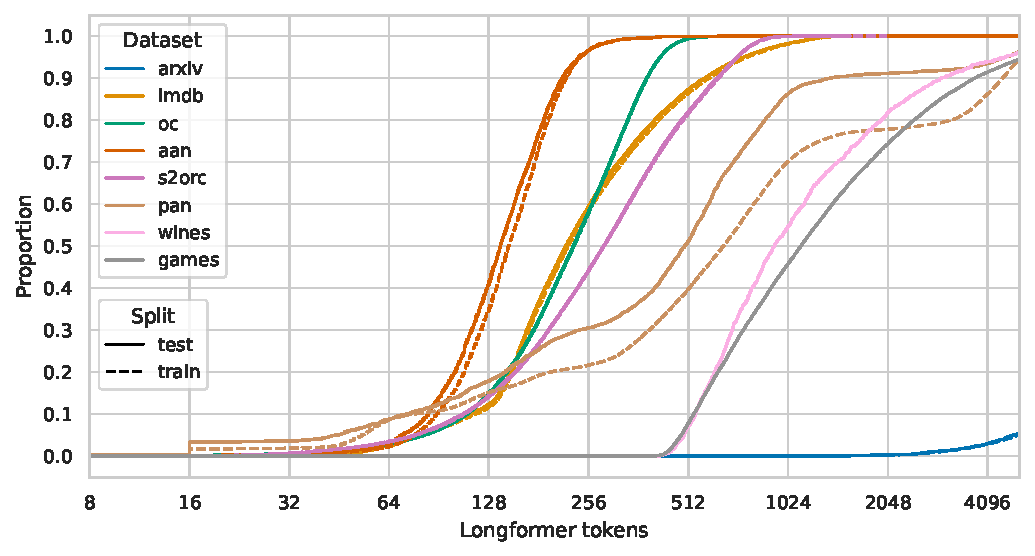
\includegraphics[width=\textwidth]{./img/eval_tasks_token_ecdf.pdf}

    \caption{Estimated cumulative length distribution of the number of
    Longformer tokens in a document.}

    \label{fig:eval_tasks_length_dist}
\end{figure}

\subsection{Tasks' description}

\paragraph{IMDB movie reviews.} The IMDB dataset~\citep{maas2011learning}
(denoted as \Task{imdb}) is a binary classification dataset frequently used to
evaluate long-context NLP models~\citep{zaheer2020big, beltagy2020longformer,
le2014distributed}. The dataset consists of movie reviews, each with an
associated rating on a 10-point scale. The reviews that rated the movie with 7
points or higher are classified as positive, and reviews with less than 4
points are classified as negative. There can be up to 30 reviews for each
movie, and the test set contains a disjoint set of movies. Along with the train
and test splits, the dataset contains an unsupervised split without rating or
class labels.

\paragraph{Arxiv papers.} Arxiv papers~\citep{arxiv_papers} (denoted as
\Task{arxiv}) is a collection of papers from ArXiv (\url{arxiv.org}),
an online archive of scholarly papers. Each paper contains its text truncated
to 10000 words but spanning at least 1000 words. The papers are classified into
11 groups based on the scientific field of the given paper. Since each paper
can be associated with several scientific fields, a small portion of the
documents ($\approx$~3.1\%) appear more than once but with different labels.
The scientific fields cover mainly fields of Computer science, such as
Artificial intelligence or Data structures, but also fields connected with
Mathematics, such as Group theory or Statistics theory.

\paragraph{ACL Anthology Network Corpus citations.} The ACL Anthology Network
Corpus citations dataset~\citep{zhou2020multilevel} (denoted as \Task{aan}) is
a citation prediction dataset. Each example in the dataset contains a pair of
paper abstracts and is classified as positive if the first document cites the
second one or negative if it does not. The dataset is compiled from the ACL
Anthology Network Corpus~\citep{radev2013acl}, where each source paper creates
positive pairs with all cited papers and a negative pair with one other randomly
sampled non-cited paper.

\paragraph{Semantic Scholar Open Corpus citations.} The Semantic Scholar Open
Corpus citations dataset~\citep{zhou2020multilevel} (denoted as \Task{oc}) is
also a citation prediction dataset in the same format as \Task{aan}. As the
dataset name suggests, it was compiled from the Semantic Scholar Open
Corpus~\citep{bhagavatula2018content}. In this dataset, only a single positive
pair is generated for each source paper, resulting in a much higher count of
unique papers compared to \Task{aan}.

\paragraph{PAN plagiarism detection.} The next classification dataset is the
PAN plagiarism detection dataset~\citep{zhou2020multilevel} (denoted as
\Task{pan}). It was constructed from PAN plagiarism alignment
task~\citep{potthast2013overview}, which is a collection of pairs of web
documents, where the sections relevant to plagiarism are humanly annotated both
in the source as well as in the suspicious document. \Task{pan} is a binary
classification task where each document pair is classified as positive or
negative. Positive inputs contain the source's plagiarised section, with a part of
the suspicious document containing the corresponding plagiarised section.
Negative pairs are constructed from the positives by replacing the source's
segment with a different part of the same document that is not annotated as being
plagiarised.

\paragraph{Semantic Scholar Open Research Corpus citations.} The Semantic
Scholar Open Research Corpus citations dataset~\citep{zhou2020multilevel}
(denoted as \Task{s2orc}) is our third and final citation prediction dataset.
The source of this dataset is the Semantic Scholar Open Research
Corpus~\citep{lo2019s2orc}, where each paper is divided into sections
connected via links to the papers cited within the given section. This structure is
used to generate positive and negative pairs. A section is paired with an
abstract of a cited paper to create a positive pair or an abstract of
a non-cited paper to create a negative pair.


\paragraph{Wines and Video games Wikipedia articles.} Both of our
similarity-based tasks are datasets consisting of Wikipedia articles from two
fields of interest: wines (denoted as \Task{wines}) and video games (denoted
as \Task{games})~\citep{ginzburg2021self}. Each dataset contains around 90
source articles, each associated with around nine similar articles. We find the two
datasets unique as they combine two aspects that are rarely seen together. First, the
similarities are based on expert human annotations, not proxy measures
such as common citations or outgoing links. Second, the documents are
relatively long, with around 90\% of documents being longer than 512 tokens.
While \Task{wines} contains fewer documents and covers fewer topics, the
similarities between a source and a target document are less apparent as it is
often based on a few details mentioned throughout the document.

\section{Results}\label{section:eval_results}

This section evaluates the student models on the previously mentioned tasks. To
put the performance of the student models into context, we compare them to four
baselines. First, to estimate the contribution of our training method, we
compare the students to their base checkpoint, Longformer, with a mean pooling
layer over its last hidden states. We also include the performances of the two
contextual teachers \Model{PV} and \Model{DM} and the structural teacher SBERT.
These models showcase the potential of our method. Ideally, we would like the
student models to combine knowledge from all their teachers and surpass all of
them. We evaluate all embedding models without any finetuning. With finetuning
on each task, the models' performance also depends on the used finetuning
method, which makes it more difficult to estimate the contribution of our
training method.

As a classifier, we use a heavily regularized neural network. We train the
classifier with cross-entropy loss for several epochs. We list the complete
list of training hyperparameters in Table~\ref{table:head_train_eval_params}.
We assess the performance of a model based on micro or binary accuracy,
depending on the number of classes. We use micro-averaging for tasks with more
classes to give each input the same weight. When we compare embedding models
across several tasks, we use \emph{normalized accuracy}, which we define in
Section~\ref{section:validation_tasks}.

\begin{table}
  \footnotesize
  \centering

  \begin{tabular}{l c}
    \toprule
    Parameter & Value \\
    \midrule
    Hidden features & 50 \\
    Hidden dropout rate & 0.5 \\
    Hidden activation & ReLU \\
    Epochs & 10 \\
    Batch size & 32 \\
    Weight decay & 0.1 \\
    Label smoothing & 0.1 \\
    Learning rate & 1e-4 \\
    Learning rate decay & Cosine \\
    Maximum gradient norm & 1.0 \\
    Optimizer & AdamW \\
    Mixed-precision training & Yes \\
    \bottomrule
  \end{tabular}

  \caption{Training parameters of classification heads during evaluation.}

  \label{table:head_train_eval_params}

\end{table}

We evaluate the classification tasks in three rounds. In each round, we limit
the number of documents on which the classifier is trained. We find that
evaluating the student models with varying amounts of finetuning data presents
a more detailed picture of the students' performances and highlights the
strengths and limitations of our training method. In the first round, we limit
the finetuning documents to 1 thousand. With so few finetuning documents, the
features that help the classifier predict the correct label must be obvious. In
this setting, models that encode only a few main features of their input should
achieve the best results. In the second round, we increase the number of
finetuning documents to 10 thousand. Finally, in the last round, we do not
limit the amount of finetuning data at all. With more finetuning data, the classifiers
can pick up on more complex features. Therefore, in the last round, models that
compress as much information as possible into their embedding should, in
theory, achieve the best results. Contrary to the evaluations in
Chapter~\ref{chapter:experiments}, we do not limit the number of test
documents. Thus, any overfitting, even with severely limited finetuning data, should be obvious. When truncating the training splits, we downsample it following its label distribution. So, the
downsampled training splits have almost equal class distribution to the
original split.

For retrieval tasks, we measure the embedding's proximity with cosine distance.
As we do not do any training, we use the whole dataset for evaluation. We
measure the models' performances based on Mean Average Precision (\emph{MAP})
but also present Mean Reciprocal Rank (MRR). While MAP scores the entire
predicted ordering, MRR is more interpretable and can be more important in
scenarios where we only care about the first positive result. When we compare
models across both tasks, we use \emph{normalized MAP}, which is computed
similarly to normalized accuracy.

We show an overview of the models' performances in
Table~\ref{table:final_evals}.

\begin{table}
  \begin{subtable}{\textwidth}
    \footnotesize
    \centering
    \begin{tabular}{lrrrrrrrr}
    \toprule
      Model & \Task{arxiv} & \Task{imdb} & \Task{aan} & \Task{oc} & \Task{pan} & \Task{s2orc} & Mean & Norm. mean \\
      \midrule
      \multicolumn{9}{c}{1k finetuning documents} \medskip \\
      Longformer                  &         .252 & \textbf{.835}&         .509 &         .655 &         .602 &         .677 &         .588 &         .814 \\
      \TableModel{DM}             &         .215 &         .591 &         .508 &         .567 &         .675 &         .581 &         .523 &         .735 \\
      \TableModel{PV}             &         .640 &         .779 &         .511 &         .654 & \textbf{.677}&         .661 &         .654 &         .918 \\
      SBERT                       &         .606 &         .780 &         .514 &         .601 &         .565 &         .605 &         .612 &         .860 \\
      \TableModel{cosine-masked}  &         .584 &         .726 &         .529 &         .747 &         .658 &         .703 &         .658 &         .922 \\
      \TableModel{MSE-contextual} & \textbf{.645}&         .762 &         .541 & \textbf{.770}&         .629 &         .733 & \textbf{.680}& \textbf{.953}\\
      \TableModel{only-MSE}       &         .642 &         .746 & \textbf{.545}&         .763 &         .635 & \textbf{.750}& \textbf{.680}& \textbf{.953}\\
      \midrule
      \multicolumn{9}{c}{10k finetuning documents} \medskip \\
      Longformer                  &         .508 & \textbf{.892}&         .521 &         .742 &         .660 &         .770 &         .682 &         .837 \\
      \TableModel{DM}             &         .650 &         .699 &         .520 &         .683 &         .695 &         .697 &         .657 &         .813 \\
      \TableModel{PV}             & \textbf{.821}&         .852 &         .537 &         .771 &         .585 &         .771 &         .723 &         .885 \\
      SBERT                       &         .785 &         .872 &         .544 &         .787 &         .599 &         .786 &         .729 &         .893 \\
      \TableModel{cosine-masked}  &         .747 &         .821 &         .568 &         .865 &         .629 &         .868 &         .750 &         .918 \\
      \TableModel{MSE-contextual} &         .752 &         .826 & \textbf{.630}&         .886 &         .702 &         .901 &         .783 & \textbf{.963}\\
      \TableModel{only-MSE}       &         .748 &         .821 &         .619 & \textbf{.892}& \textbf{.717}& \textbf{.904}& \textbf{.784}& \textbf{.963}\\
    \midrule
      \multicolumn{9}{c}{All finetuning documents} \medskip \\
      Longformer                  &         .649 & \textbf{.913}&         .625 &         .889 &         .675 &         .899 &         .775 &         .894 \\
      \TableModel{DM}             &         .710 &         .731 &         .570 &         .835 &         .685 &         .835 &         .728 &         .843 \\
      \TableModel{PV}             & \textbf{.840}&         .865 &         .703 &         .891 &         .602 &         .899 &         .800 &         .923 \\
      SBERT                       &         .819 &         .890 & \textbf{.805}& \textbf{.935}&         .640 & \textbf{.944}& \textbf{.839}& \textbf{.969}\\
      \TableModel{cosine-masked}  &         .779 &         .843 &         .751 &         .918 &         .638 &         .925 &         .809 &         .935 \\
      \TableModel{MSE-contextual} &         .776 &         .842 &         .767 &         .930 &         .720 &         .942 &         .829 &         .961 \\
      \TableModel{only-MSE}       &         .773 &         .837 &         .760 &         .929 & \textbf{.740}&         .941 &         .830 &         .962 \\
    \bottomrule
    \end{tabular}

    \caption{Classification tasks}

    \label{table:final_evals_cls}

  \end{subtable}
  \bigskip

  \begin{subtable}{\textwidth}
    \footnotesize
    \centering
    \begin{tabular}{lrrrr}
      \toprule
      Model & \Task{games} & \Task{wines} & Mean & Norm. mean \\
      \midrule
      Longformer                  &         .158 &         .096 &         .127 &         .724 \\
      \TableModel{DM}             &         .130 &         .115 &         .123 &         .717 \\
      \TableModel{PV}             &         .173 &         .133 &         .153 &         .887 \\
      SBERT                       &         .191 &         .143 &         .167 &         .964 \\
      \TableModel{cosine-masked}  &         .165 & \textbf{.148}&         .157 &         .917 \\
      \TableModel{MSE-contextual} &         .186 &         .145 &         .165 &         .957 \\
      \TableModel{only-MSE}       & \textbf{.198}&         .145 & \textbf{.172}& \textbf{.989}\\
      \bottomrule
    \end{tabular}

    \caption{Retrieval tasks}

  \end{subtable}

  \caption{Performance of evaluated embedding models on all downstream tasks.
  For classification tasks, we show the performance with all finetuning data
  and with only 1k and 10k finetuning documents. For classification tasks, we
  show binary or micro accuracy. For retrieval tasks, we show MAP. We also
  display the mean score and the mean of normalized scores for each model.}

  \label{table:final_evals}

\end{table}

\subsection{Classification tasks}\label{section:eval_cls_tasks}

We evaluate the embedding models' performance on the classification tasks in
three rounds. First, we compare the overall performance of the models between
the three different rounds. Then, we explore the models' performances per task
in detail.

First, we focus on the overall models' performance throughout the three
evaluation rounds, which we present in Figure~\ref{fig:final_eval_norm_all}.
The relative performance of the baselines and student models is similar to what
we witness in Chapter~\ref{chapter:experiments}. In the first two rounds, the
students outperform all baselines. In the last round, they beat all contextual
teachers and improve the score of Longformer. However, they are only just worse
than SBERT. The best student is {\OnlyMSEStudent} followed by {\MSEStudent}. We
witness the same order of corresponding models on validation tasks at the end
of Chapter~\ref{chapter:experiments}. However, as {\CosineStudent} is trained
with the structural loss only on short inputs, it receives 3.26 times fewer
update steps with the structural loss than the other two students.
Consequently, {\CosineStudent} often outperforms its contextual teacher only by
a fraction, creating a noticeable performance gap between it and the other two
students.

\begin{figure}

  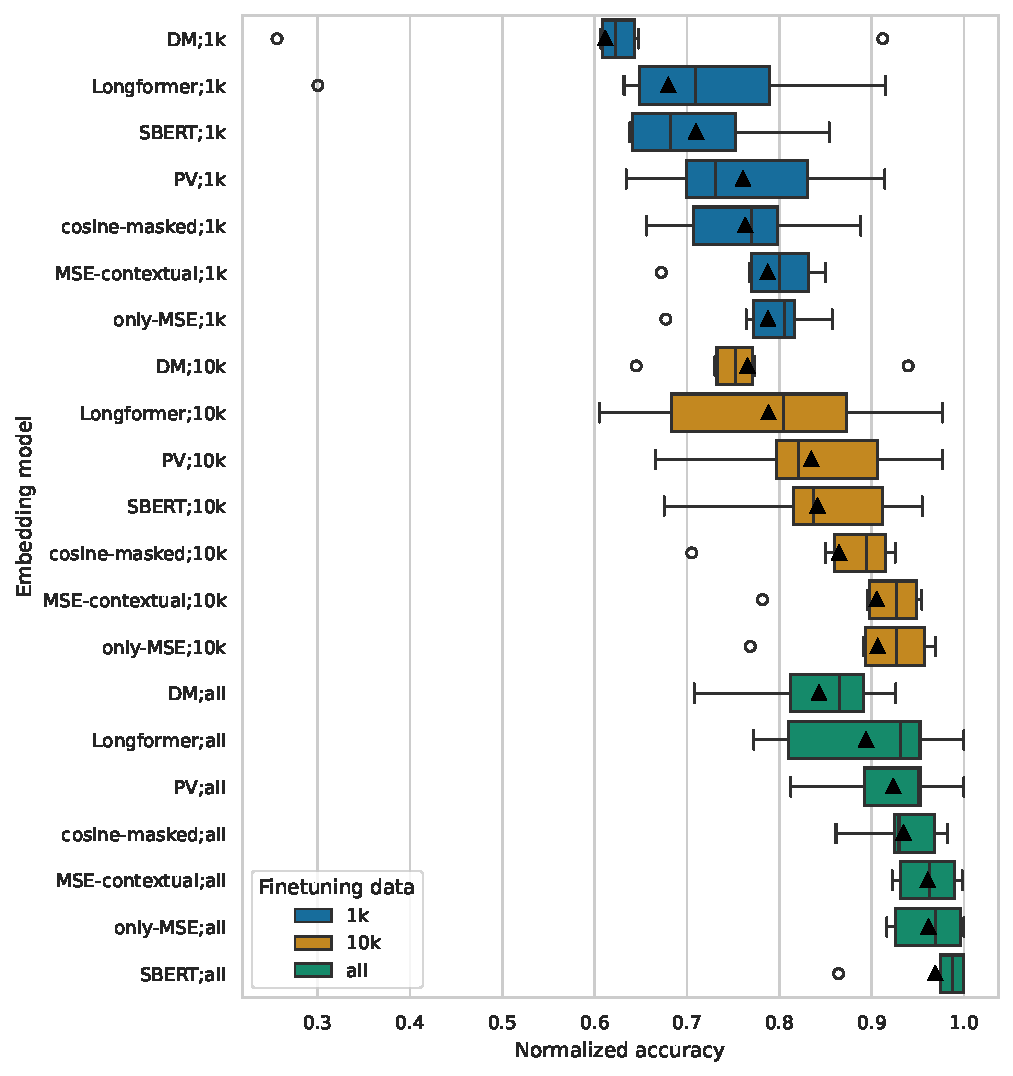
\includegraphics[width=\textwidth]{img/final_eval_norm_all.pdf}

  \caption{Overall relative performance of embedding models throughout the three
  rounds. In the first two rounds, we limit the number of finetuning documents to 1k
  and 10k, but do not set any limit in the third round labeled as ``all''.}

  \label{fig:final_eval_norm_all}

\end{figure}

In the first round, Longformer's and SBERT's performance is underwhelming. At
the same time, the best student model achieves, on average, nearly 80\% of the
best performance for a given task achieved by an embedding model with all
finetuning data. We see this as a considerable achievement since there are 17
to 240 times more finetuning documents in the last round compared to the first
one. In the second round, the classifiers are trained on 10k finetuning
documents, and their performances naturally increase. Particularly for SBERT, as
it now surpasses \Model{PV}, which improves by a relatively small amount. These
effects are also noticeable in the performance of {\CosineStudent} as there is
a more significant gap between it and the other two students that rely on
SBERT more. Finally, with all finetuning data, the differences between models'
performances diminish as the best models improve only marginally. SBERT takes
the greatest advantage of the increase in finetuning data and surpasses all
other models. We see this as a demonstration that the embedding model does not
strictly need a large maximum context for the selected set of tasks. In other
words, despite the moderately large documents, we can reach a competitive
performance by only considering the first 384 tokens of each input. This is
apparent, especially for \Task{arxiv}, where we can imagine classifying the
field of a scholarly paper based on just its abstract. So, as the context is of
minor importance, SBERT benefits from its full attention and surpasses the best
student by a small fraction. Nonetheless, all student models can improve the
scores of their contextual teachers and base checkpoints. Moreover, the
students reach consistent and comparable performances despite being trained
differently. {\CosineStudent} trains with a different contextual teacher,
contextual loss, structural loss, and weighting of the two losses than the rest
of the students. {\MSEStudent} trains with a significantly less performant
contextual teacher, while {\OnlyMSEStudent} does not use a contextual teacher.
This shows that our method is robust and open to multiple changes in various
aspects.

We now examine the models' performances per each task, which we plot in
Figure~\ref{fig:final_cls_evals}. The relative models' performances on a given
task stay consistent throughout the three rounds, so we focus only on the last
two. With 10k finetuning documents, the students perform best on
classifications of document pairs. On \Task{imdb}, Longformer shows the best
performance, which is surprising given it is the second-worst model in both
rounds. On \Task{arxiv}, PV shows the best performance as it benefits from its
large embedding and unlimited context. Arguably, both of these attributes play
a role, as \Model{DM} with the same unlimited context but with more than 50
times smaller embedding performs better than Longformer but worse than
\Model{PV}. As we increase the number of finetuning documents, SBERT
substantially improves. We register the largest performance increase for tasks
with the most finetuning data available. These are \Task{aan}, \Task{oc}, and
\Task{s2orc}. We also highlight SBERT's performance on \Task{arxiv} in both
rounds, where it outperforms all students with eight times larger maximum
context and comes relatively close to the performance of \Model{PV}. This
demonstrates that, despite the task being composed of only very long documents,
we can achieve a competitive performance based on just the first few hundred
tokens. The insignificance of an embedding model's lack of context may partly
explain why the students' performances for a given task are not affected by the
length of the tasks' documents. For example, on tasks with longer documents
such as \Task{arxiv} or \Task{pan}, {\CosineStudent} and {\MSEStudent} perform
on par with {\OnlyMSEStudent} despite being trained with a contextual teacher,
which should theoretically improve the students' performance on longer inputs.

\begin{figure}

  \centering
  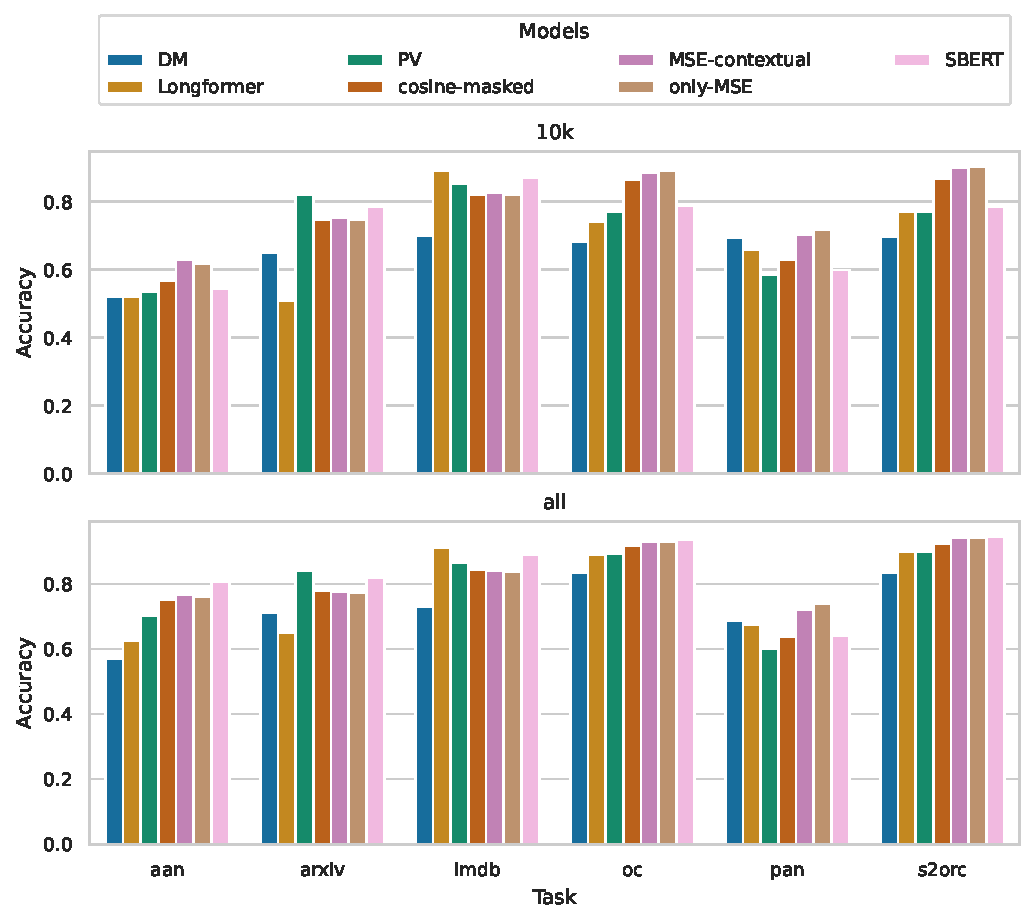
\includegraphics[width=\textwidth]{img/final_cls_evals.pdf}

  \caption{Performance of embedding models on evaluation tasks with the finetuning documents being limited to 10k and with all finetuning data.}

  \label{fig:final_cls_evals}

\end{figure}

\subsection{Retrieval tasks}

\begin{figure}[p]

  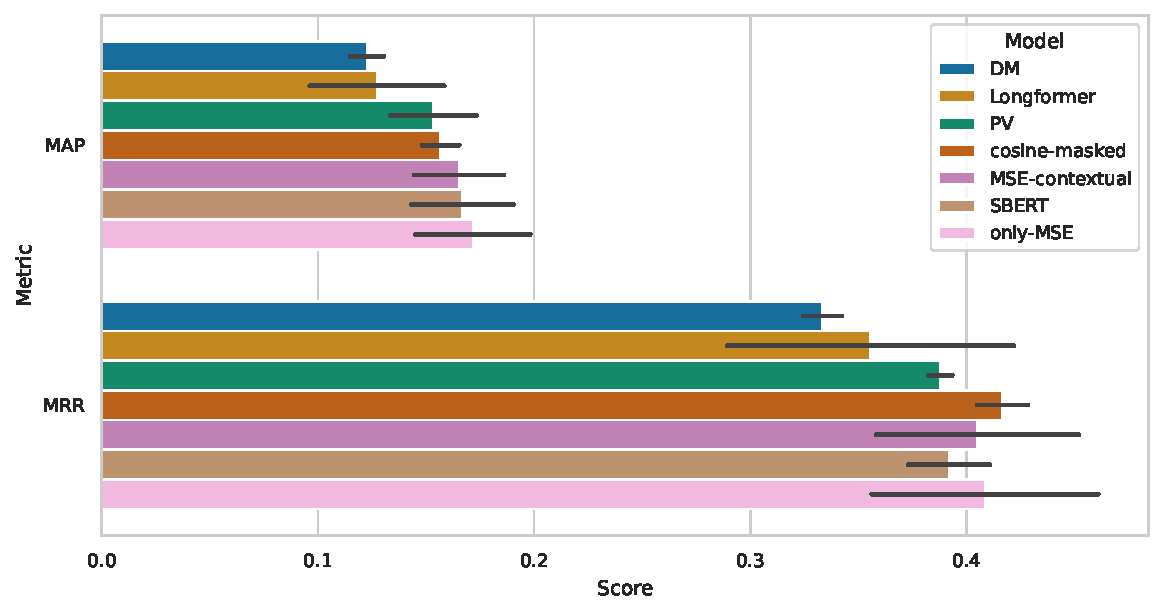
\includegraphics[width=\textwidth]{img/final_sims_evals.pdf}

  \caption{Performance of models on retrieval tasks. We mark the mean score
  with a bar and the span between each task's score with an error bar.}

  \label{fig:final_eval_sims}

\end{figure}

\begin{figure}[t]

  \centering
  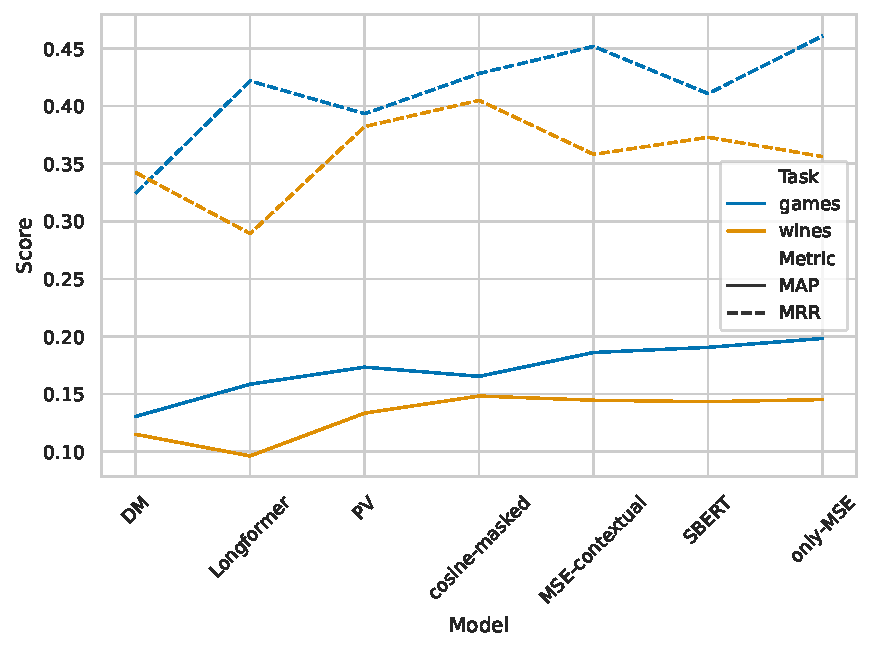
\includegraphics[width=0.85\textwidth]{img/final_sims_evals_per_task.pdf}

  \caption{Performance of embedding models on each retrieval task.}

  \label{fig:final_eval_sims_per_task}

\end{figure}

We plot the overall models' performances on the retrieval tasks in
Figure~\ref{fig:final_eval_sims}. In terms of MAP, the best-performing model is
{\OnlyMSEStudent} closely followed by SBERT and the other two student models.
For Mean Reciprocal Rank, the best model is {\CosineStudent}, one
of the most consistent models in both metrics. This suggests that using
a structural teacher only for inputs, which it can process as a whole, may lead to a
more consistent student model.


We also plot the models' performances per each task in
Figure~\ref{fig:final_eval_sims_per_task}. As the results suggest, \Task{games}
is an easier task than \Task{wines}. This may be unexpected since, compared to
\Task{wines}, \Task{games} has more total documents but a similar amount of
source and target documents. Consequently, \Task{games} contains much more
``noise'' documents, which may hurt the performance. However, as we mention in
the tasks' description, the selection of topics for \Task{games} is much wider,
and the differences between documents are far less nuanced. On the other hand,
the similarities of documents in \Task{wines} are sometimes based on a few
details mentioned throughout the document.

\chapter*{Conclusion}
\addcontentsline{toc}{chapter}{Conclusion}


%%% Bibliography
%%% Bibliography (literature used as a source)
%%%
%%% We employ bibTeX to construct the bibliography. It processes
%%% citations in the text (e.g., the \cite{...} macro) and looks up
%%% relevant entries in the bibliography.bib file.
%%%
%%% The \bibliographystyle command selects, which style will be used
%%% for references from the text. The argument in curly brackets is
%%% the name of the corresponding style file (*.bst). Both styles
%%% mentioned in this template are included in LaTeX distributions.

\bibliographystyle{plainnat}    %% Author (year)
% \bibliographystyle{unsrt}     %% [number]

\renewcommand{\bibname}{Bibliography}

%%% Generate the bibliography. Beware that if you cited no works,
%%% the empty list will be omitted completely.

\bibliography{bibliography}

\bigskip
\noindent
For final corrections we used Grammarly (\url{grammarly.com}).

%%% If case you prefer to write the bibliography manually (without bibTeX),
%%% you can use the following. Please follow the ISO 690 standard and
%%% citation conventions of your field of research.

% \begin{thebibliography}{99}
%
% \bibitem{lamport94}
%   {\sc Lamport,} Leslie.
%   \emph{\LaTeX: A Document Preparation System}.
%   2nd edition.
%   Massachusetts: Addison Wesley, 1994.
%   ISBN 0-201-52983-1.
%
% \end{thebibliography}


%%% Figures used in the thesis (consider if this is needed)
\listoffigures

%%% Tables used in the thesis (consider if this is needed)
%%% In mathematical theses, it could be better to move the list of tables to the beginning of the thesis.
\listoftables

%%% Abbreviations used in the thesis, if any, including their explanation
%%% In mathematical theses, it could be better to move the list of abbreviations to the beginning of the thesis.
% \chapwithtoc{List of Abbreviations}

%%% Attachments to the master thesis, if any. Each attachment must be
%%% referred to at least once from the text of the thesis. Attachments
%%% are numbered.
%%%
%%% The printed version should preferably contain attachments, which can be
%%% read (additional tables and charts, supplementary text, examples of
%%% program output, etc.). The electronic version is more suited for attachments
%%% which will likely be used in an electronic form rather than read (program
%%% source code, data files, interactive charts, etc.). Electronic attachments
%%% should be uploaded to SIS and optionally included in the thesis on a~CD/DVD.
%%% Allowed file formats are specified in the provision of the rector no. 72/2017.
\appendix
\chapter{Attachments}

% \section{First Attachment}

\openright
\end{document}
